\chapter{Реализация и экспериментальная проверка}

В данной главе приводятся детали разработки и экспериментальной проверки
разработанной системы. Описаны результаты экспериментов для разработанной
модели сравниваются с результатами аналогичных экспериментов для существующих моделей.
Описаны данные, которые использовались в экспериментах.

\section{Состав и структура реализованного программного обеспечения}

Реализованное ПО --- это модуль на python, который позволяет помочь эксперту
исследовать моделируемую систему и структурировать знания о системе.

Так как разработка проводилась методикой Test-Driven-Development \cite{beck2003test_tdd, janzen2005test},
были написаны автотесты, которые запускаются
при обновлении кода в удаленном репозитории. Кроме автотестов,
в среде по запуску тестов проверяется качество кода и возможные ошибки
с помощью линтеров на соответствие кода стандарту $ pep8 $.
Автотесты необходимы проекту на языке с динамической типизацией,
так как в интерпретируемых языках с динамической типизацией
интерпретатор на стадии компиляции программы не может проверить или вывести, чтобы проверить
типы переменных и аргументов функций самостоятельно. Поэтому код, который
не покрыт тестами может не работать и об этом разработчик узнает
только после того, как программа упадет. Но раннее обнаружение этих
ошибок с помощью автотестов поможет избежать проблем с использованием модуля в
продакшне и поможет сократить время доведения продукта до состояния успешного релиза.
Для того, чтобы было проще искать ошибки в коде и в тестах,
тело тестов должно быть максимально простым.
Разработанные автотесты покрывают как негативные, так и позитивные
сценарии работы программы.
Для разработанного модуля было реализовано 6 автотестов:

\begin{itemize}
	\item \verb|test_fit_on_history| --- проверяет, что обучение карты на исторических данных с использованием оптимизатора $ SGD $ проходит без ошибок
	\item \verb|test_fit_on_history_with_exogen_param| --- проверяет, что обучение карты на исторических данных с использованием экзогенных параметров проходит без ошибки
	\item \verb|test_sum_model| --- проверяет, работу модели по суммированию концептов
	\item \verb|test_double_freeze| --- проверяет, что генерируется ошибка при неправильном использовании метода \verb|freeze|.
	\item \verb|test_freeze_history_mismatch| --- проверяет, что генерируется ошибка при несовпадении размерностей исторических данных в концептах
	\item \verb|test_train_lstm| --- проверяет, что обучение карты на исторических данных с использованием оптимизатора $ ADAM $ проходит без ошибок
\end{itemize}

Отчет по тестированию представлен в приложении \ref{listing:test_report}.

\section{Анализ данных}

Анализ и предобработка данных были проведены с использованием
библиотек $ pandas $ и $ statmodels $.
Набор данных, на которых будет проводиться тестирование разработанной системы
представляет из себя несколько $ csv $ файлов: файл с количеством продаж
продуктов разных категорий в 3 магазинах за 5 лет начиная с 2011-01-29
и файл с описанием праздников, которые выпадают на каждый день.

Обработка исходных данных включала в себя:

\begin{itemize}
	\item Разбивка категориальных признаков на несколько числовых (индикаторных) с помощью one-hot-encoding; % todo ref
	\item Объединение набора данных с праздниками и набора данных к продажами товаров в одну таблицу по ключевому столбцу date;
	\item Группировка исходных данных по дате с последующим суммированием  внутри группы. Это преобразование
	позволяет получить общее количество продаж за один день для заданного набора данных.
\end{itemize}

\noindent описанные преобразования производились с помощью библиотеки $ pandas $.
Описание результирующего набора данных \ref{tbl:sales_dataset_description}
и количественные характеристики \ref{tbl:sales_dataset_description_quantitive}
исследуемого набора данных представлены в приложении.

Требуется предсказать количество продаж на 30 дней вперед.

Для начала можно провести качественный визуальный анализ данных.
Общее количество продаж можно оценить на графике \ref{img:all_sales}.
Из этого графика видно, что до середины 2012 года количество проданных
товаров увеличивалось. Но после тренд пропал. В данных можно наблюдать
как годичные, так и месячные и даже недельные сезонности. Каждый год
в Рождество количество проданных товаров равно 0, потому что магазин не работает.
По выходным количество проданных товаров больше, чем в будние дни.

Количество проданных товаров по каждому магазину представлено на следующем графике \ref{img:sales_by_store}.
В количестве проданных товаров отдельно по каждому магазину нет значительных отличий.
Все магазины продают примерно одинаковое количество товаров.

Количество продаж по категориям для каждого магазина на графику \ref{img:sales_by_store_by_cat}
Во всех трех магазинах количество продаж товаров в категории "еда" больше всего,
а товаров для дома меньше всего. Из данного графика можно заметить, что сезонность
присутствует в графике по продаже товаров в категории "еда" и для товаров для дома, но
для товаров для хобби сезонности не наблюдаются.

Рассмотрим графики автокорреляции и частичной автокорреляции для общего количества продаж
\ref{img:any_autocorrelation}.
Для лагов 1, 2, 3, 6, 7 присутствует статически значимая частичная автокорреляция.
Это может быть использовано при построении модели SARIMAX.
На графики автокорреляции видны синусоидальные колебания. Это подтверждает,
что в данных есть сезонность.

Для обучения моделей использовался набор данных полностью за
исключением последних 30 точек. Оставшиеся 30 точек использовались для
валидации предсказаний исследуемых моделей.

\def\figurename{Рис}
\begin{figure}[t]
	\centering
	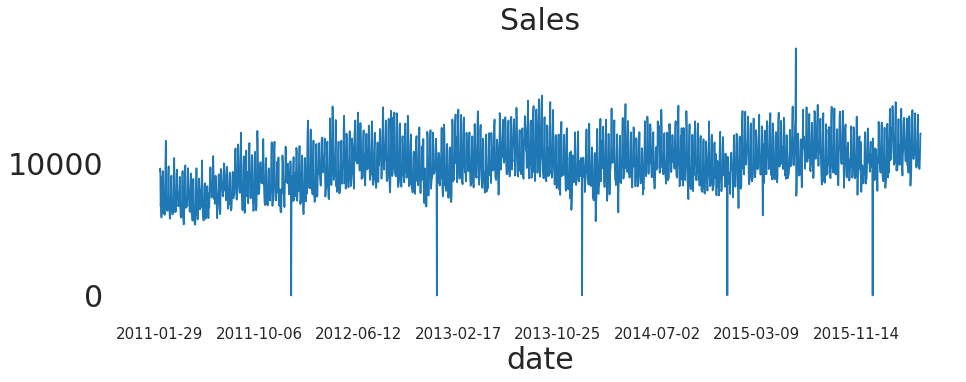
\includegraphics[width=0.9\columnwidth]{./img/all_sales.png}
	\caption{Количество продаж}
	\label{img:all_sales}
\end{figure}


\def\figurename{Рис}
\begin{figure}[t]
	\centering
	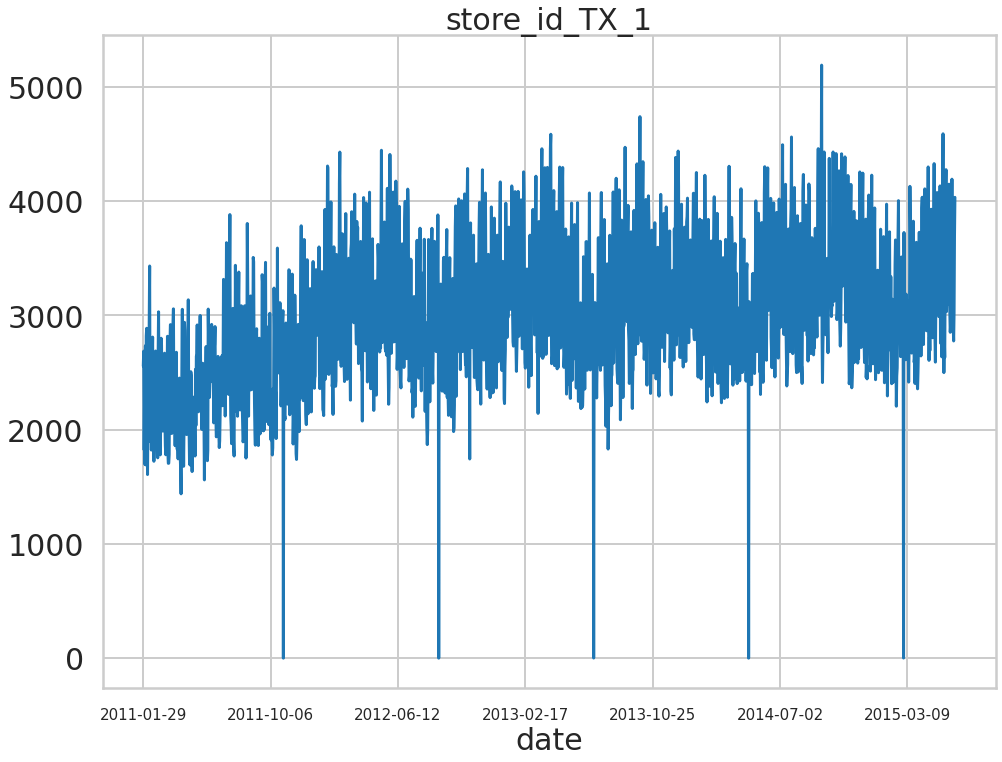
\includegraphics[width=0.25\columnwidth]{./img/store_tx1_total.png}
	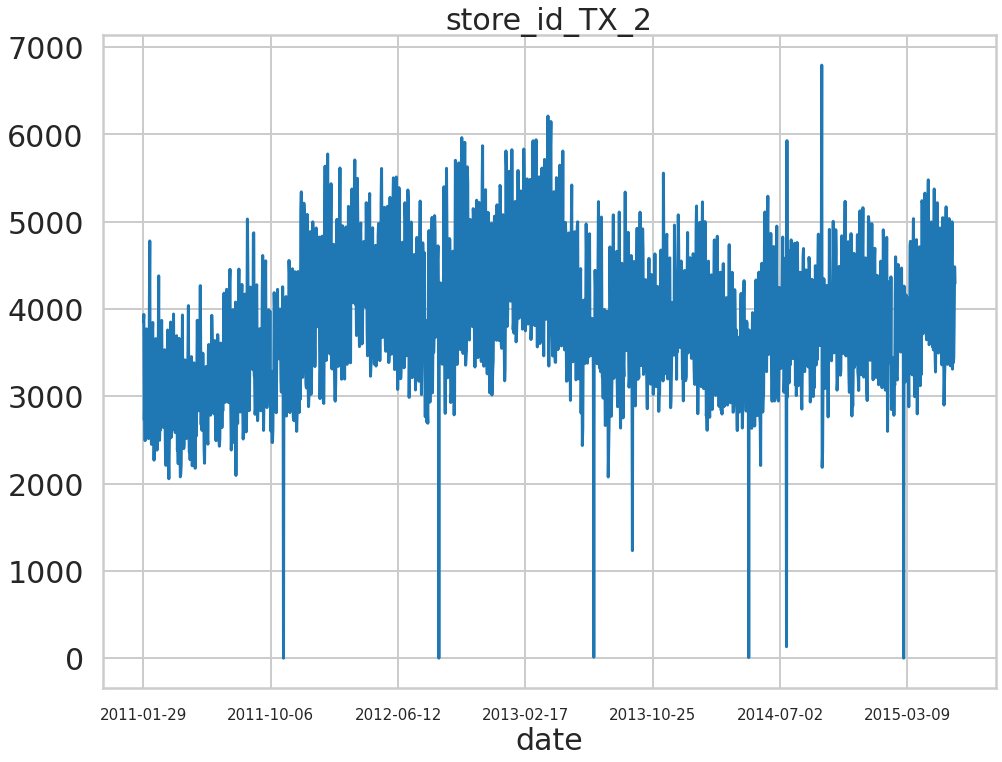
\includegraphics[width=0.25\columnwidth]{./img/store_tx2_total.png}
	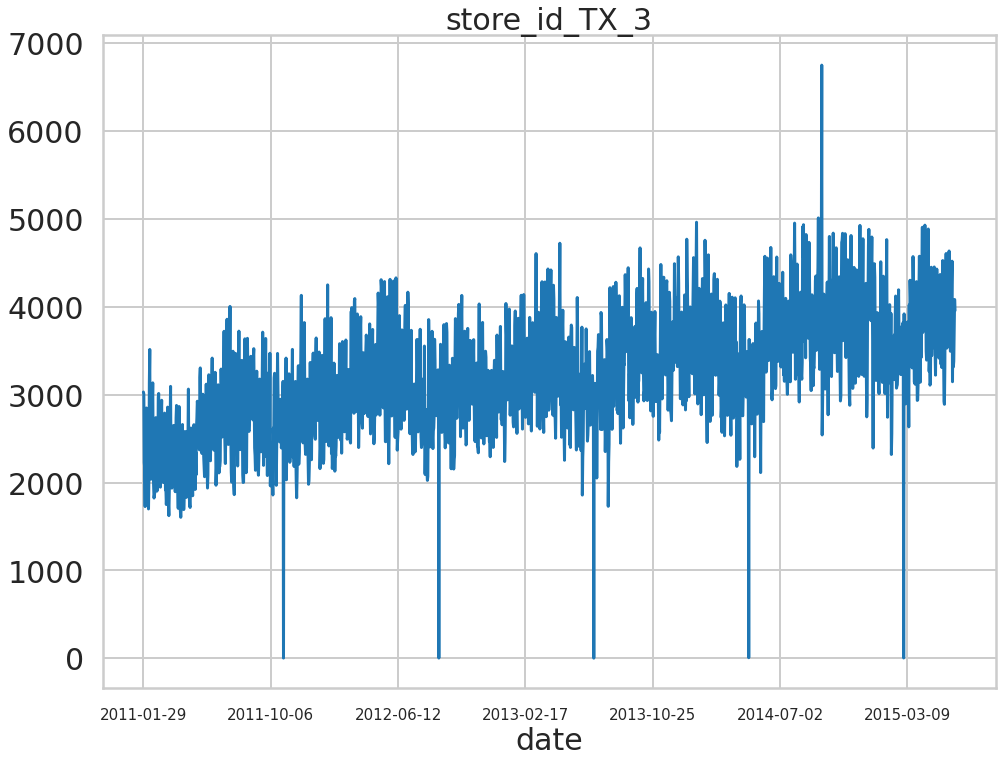
\includegraphics[width=0.25\columnwidth]{./img/store_tx3_total.png}
	\caption{Общее количество продаж по каждому магазину}
	\label{img:sales_by_store}
\end{figure}

\def\figurename{Рис}
\begin{figure}[t]
	\centering
	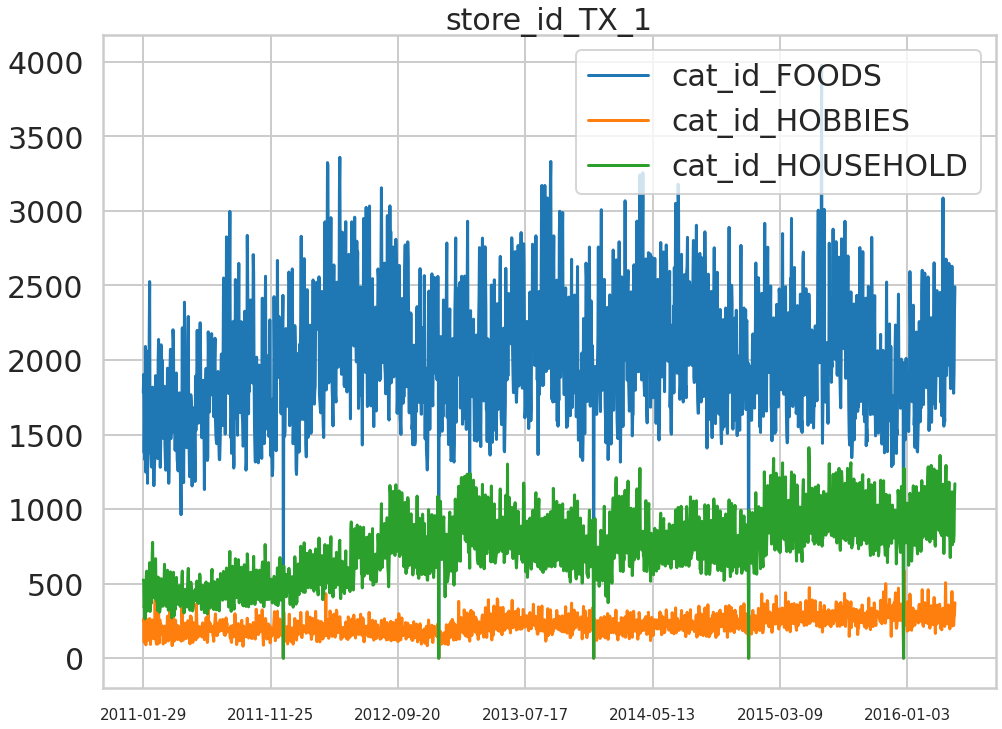
\includegraphics[width=0.25\columnwidth]{./img/store_tx1_by_cats.png}
	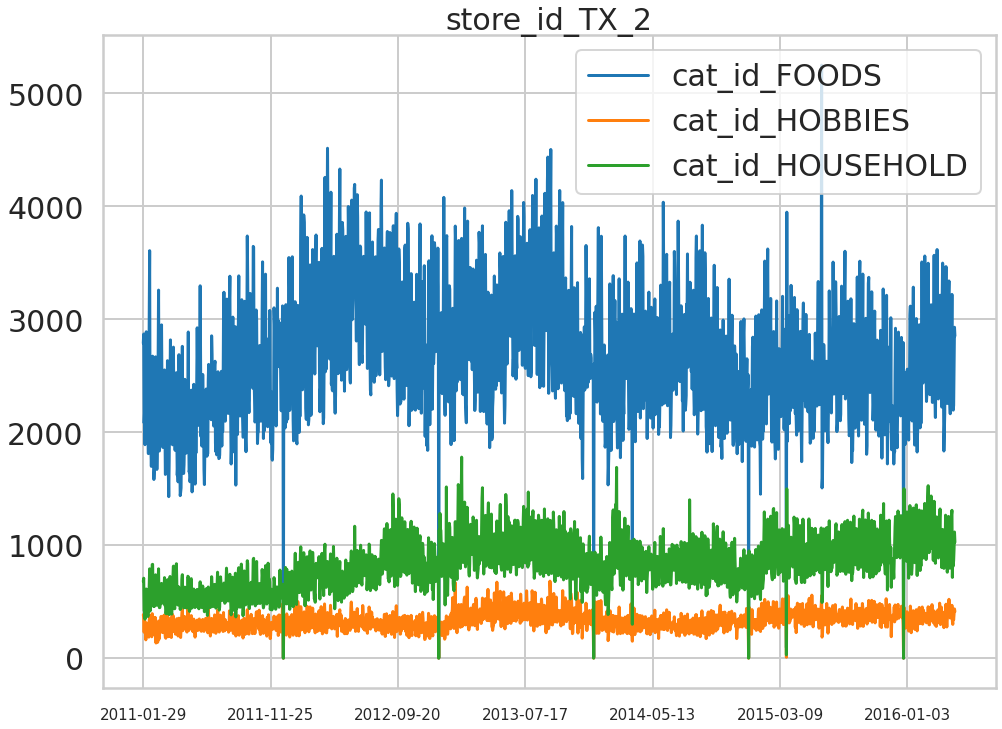
\includegraphics[width=0.25\columnwidth]{./img/store_tx2_by_cats.png}
	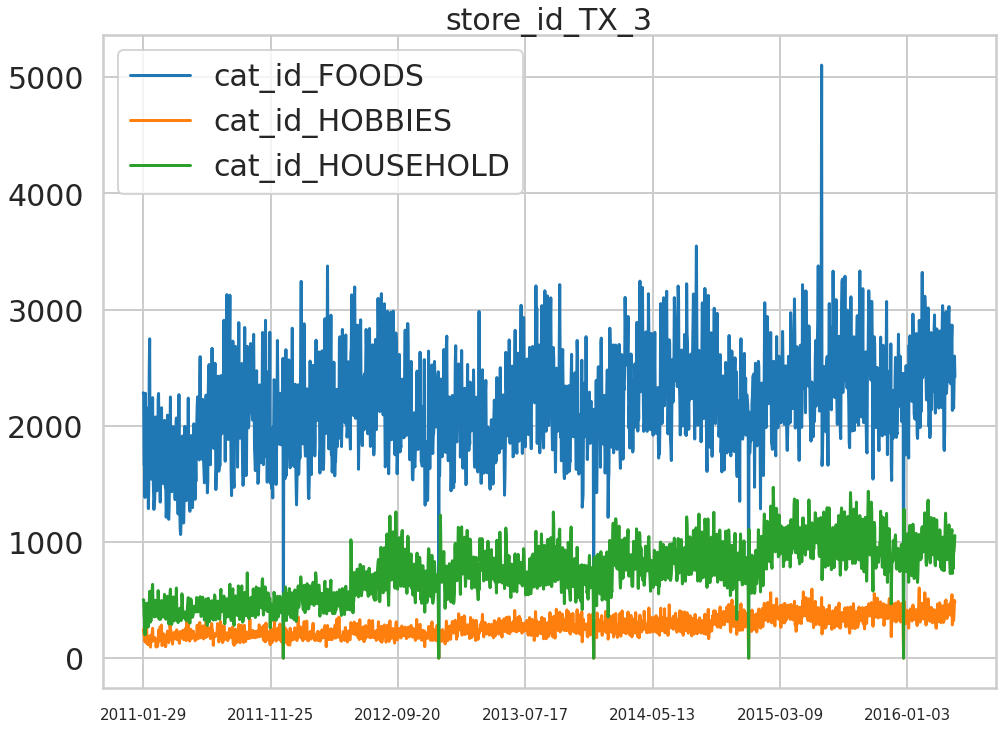
\includegraphics[width=0.25\columnwidth]{./img/store_tx3_by_cats.png}
	\caption{Количество продаж товаров определенной категории для каждого магазина}
	\label{img:sales_by_store_by_cat}
\end{figure}

\def\figurename{Рис}
\begin{figure}[t]
	\centering
	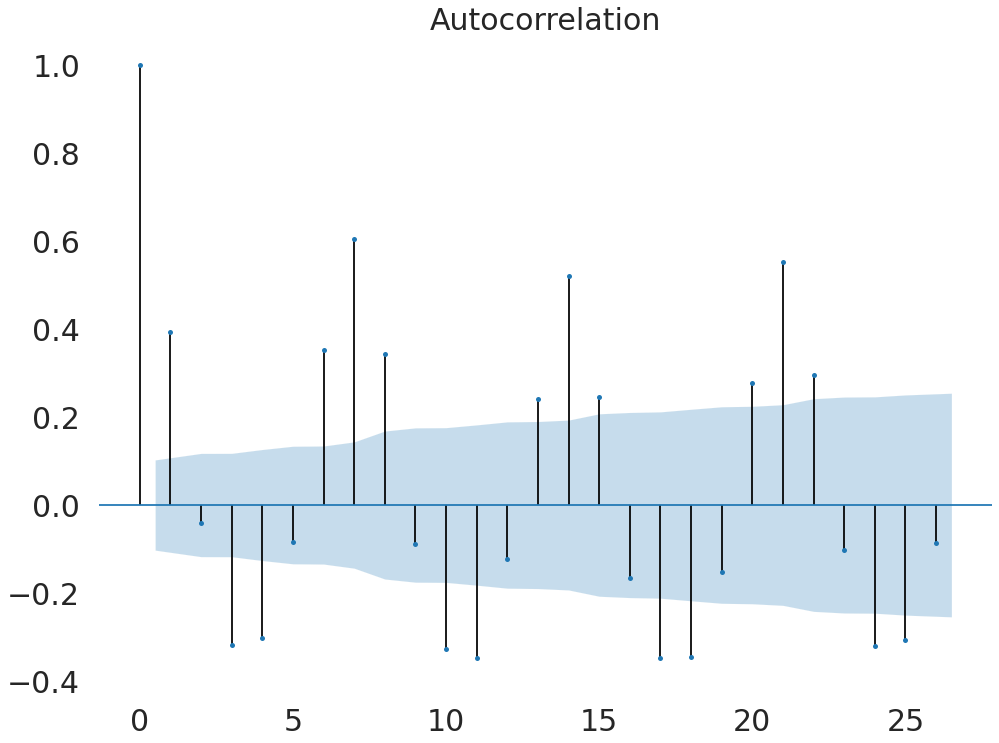
\includegraphics[width=0.4\columnwidth]{./img/sales_autocorrelation.png}
	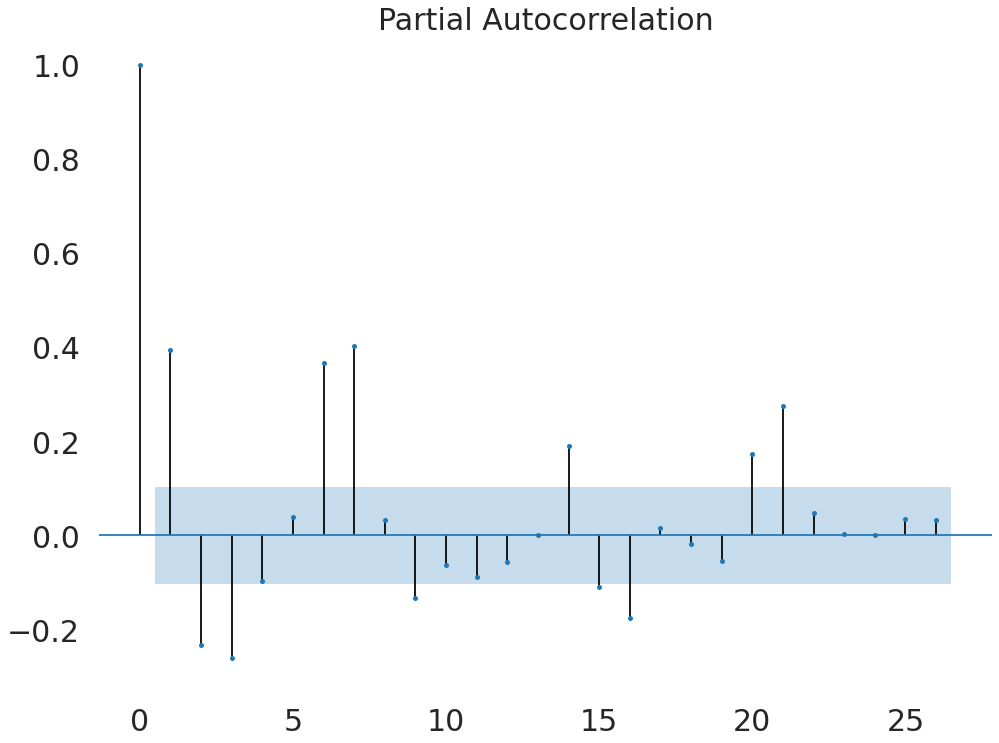
\includegraphics[width=0.4\columnwidth]{./img/sales_partial_autocorrelation.png}
	\caption{Автокорреляция и частичная автокорреляция для общего количества продаж}
	\label{img:any_autocorrelation}
\end{figure}



\section{Построение модели SARIMAX}

Данная модель разрабатывалась с использованием библиотеки $ statmodels $.
Для оптимального подбора гиперпараметров был проведен
визуальный анализ исходных данных, поиск перебором модели
с минимальным значением критерия Акаике.
Оптимизация параметров на полном наборе данных занимает примерно 10 секунд при 8 параметрах модели.

Оптимальными гиперпараметрами оказались:
\begin{equation}
	p = 2, d = 0, q = 3, P = 0, D = 1, Q = 1, S = 7
\end{equation}
\noindent Сезонность недельная  -~ это логично, что в текущий день
товаров будет продано столько же, как неделю назад.


На графике остатков \ref{img:arimax_resid} все еще прослеживается
годичная сезонность и выбросы. Данные выбросы -~ возможно предсказать, если
добавить экзогенные параметры в виде индикатора праздников.

В качестве экзогенных параметров рассмотрим индикатор дня недели.
В исходные данные добавится 7 колонок. Каждому дню недели
будет соответствовать одна колонка. И еще одним экзогенным параметром
возьмем индикатор праздника --- Рождества.
Экзогенные параметры можно вычислить заранее, так как наперед можем
поставить в соответствие индикатор дня недели определенному календарному дню
и индикатор Рождества.
Оптимизация параметров модели с 8 экзогенными переменными потребовало 20 секунд.

На графике остатков модели с экзогенными переменными \ref{img:arimax_resid} видно, что удалось избавиться
от большого значения остатков на Рождество. Это получилось сделать благодаря
столбцу-индикатору Рождественских праздников.

\def\figurename{Рис}
\begin{figure}[t]
	\centering
	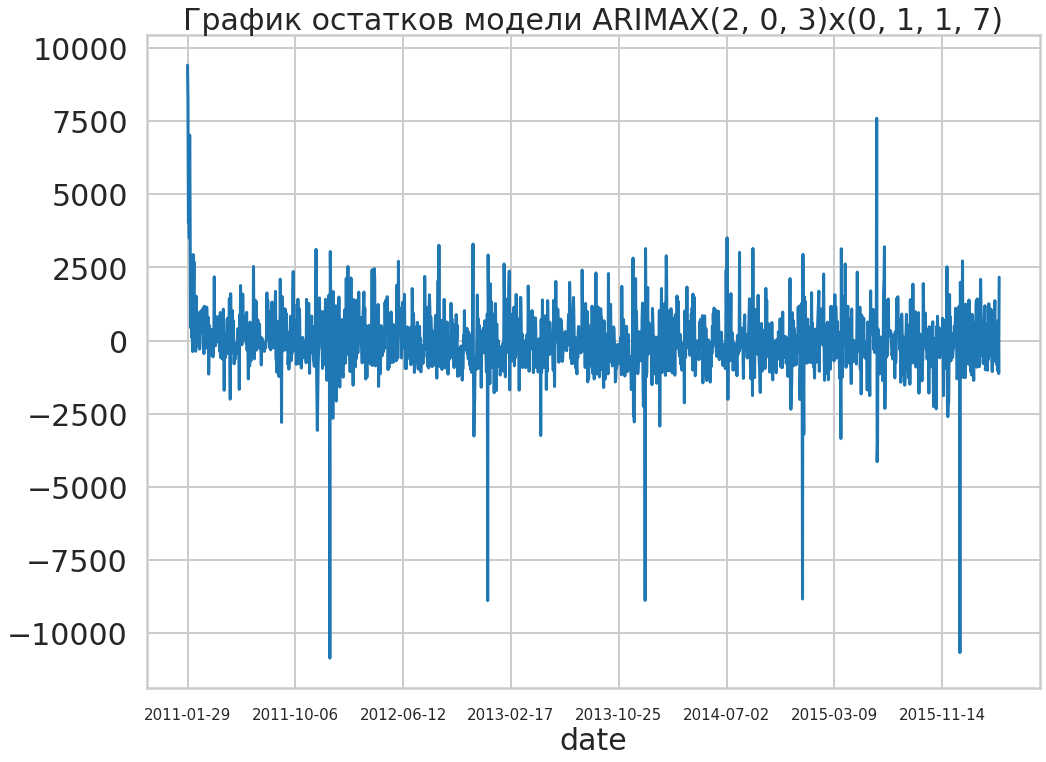
\includegraphics[width=0.4\columnwidth]{./img/arimax_resid.png}
	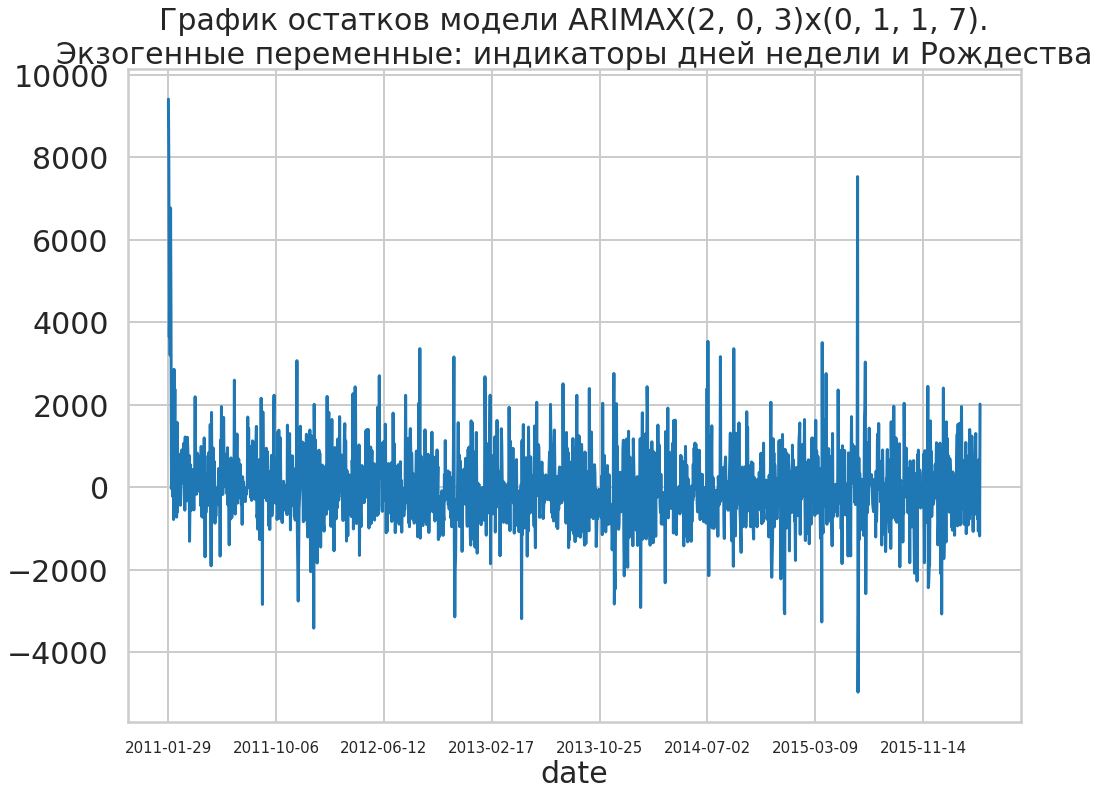
\includegraphics[width=0.4\columnwidth]{./img/arimax_resid_with_xmas.png}
	\caption{График остатков модели ARIMAX с соответствующими параметрами}
	\label{img:arimax_resid}
\end{figure}

Но если проанализировать значения коэффициентов обученной модели \ref{tbl:arimax_coeffs_exogen},
можно заметить, что индикаторы дня недели слишком слабо влияют на предсказание модели.
Значения коэффициентов очень маленькие, вероятность того, что эти параметры будут иметь
значение больше критического равно единице, дисперсия большая. Из этого можно сделать вывод,
что использование этих экзогенных переменных неоправданно. Но зато значение коэффициента
для индикатора Рождества ($ xmas $) большое. Этот экзогенный параметр
действительно объясняет некоторую полезную часть данных. Так, значение теста Харке-Бера \cite{thadewald2007jarque}
для предыдущей модели было равно $ 37658.88 $, а после выявления зависимости между количеством продаж
и днем рождества стало равно $ 1488.02 $. Чем ближе значение этого теста к нулю, тем больше остатки
модели похожи на нормальное распределение. Этот тест сверяет асимметрию и эксцесс остатков с
значениями этих моментов для нормального распределения. И хотя с таким абсолютным значением
теста нельзя говорить о том, что остатки распределены нормально, но относительно предыдущей
модели, новая модель определенно лучше.

Но на предсказании на 30 дней вперед найденные экзогенные переменные не повлияли \ref{img:arimax_forecast},
так как в исследуемый момент времени не было Рождества.

\def\figurename{Рис}
\begin{figure}[t]
	\centering
	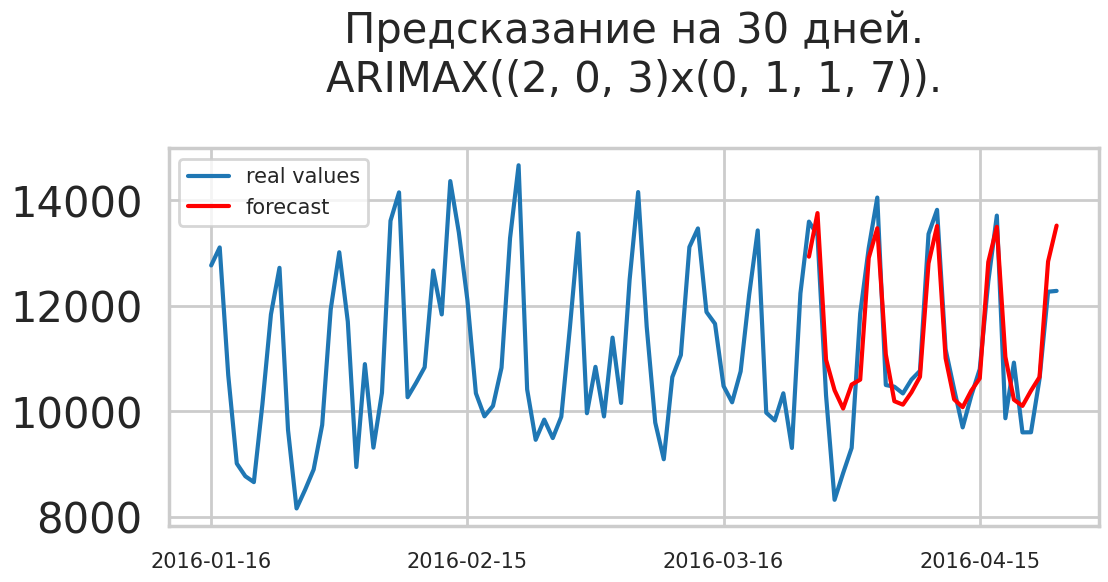
\includegraphics[width=0.9\columnwidth]{./img/arimax_simple_pred30.png}
	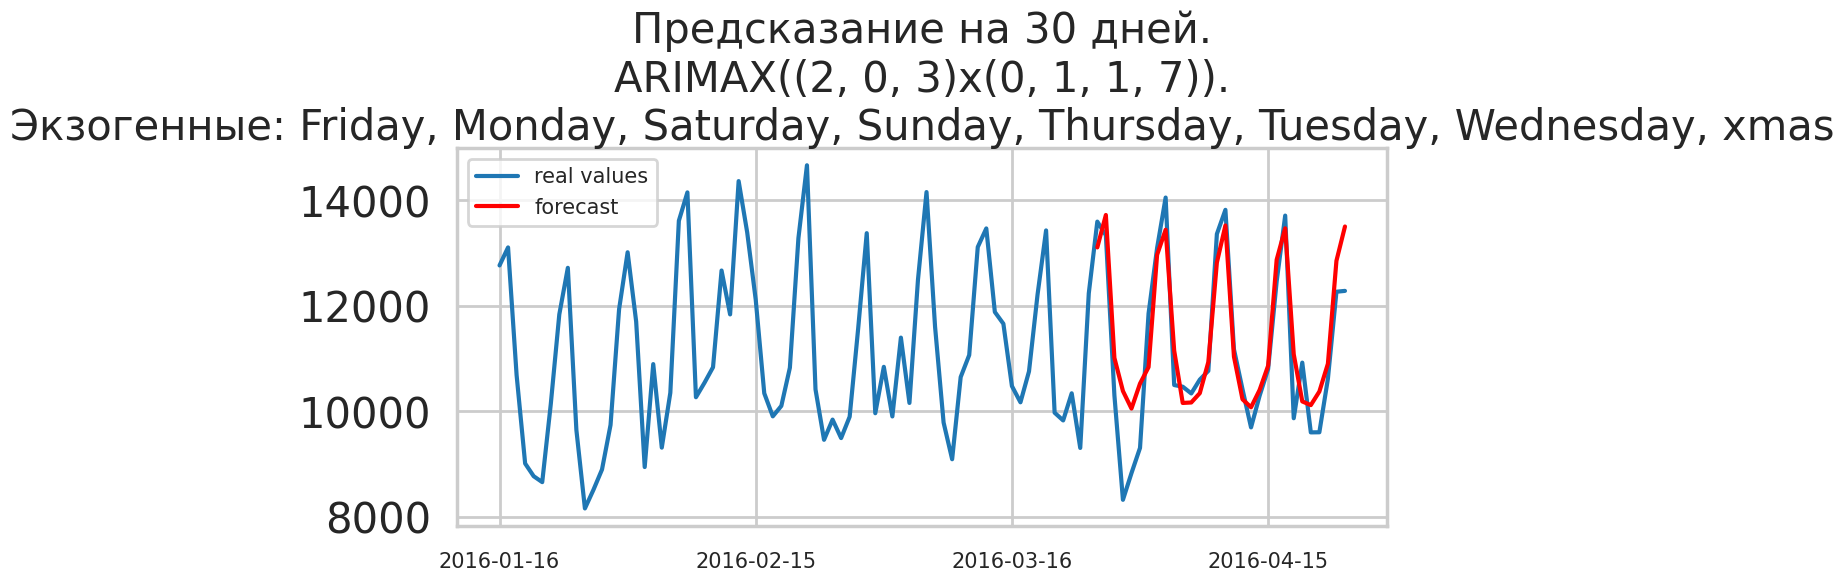
\includegraphics[width=0.9\columnwidth]{./img/arimax_with_exog_pred30.png}
	\caption{Предсказания на 30 дней вперед}
	\label{img:arimax_forecast}
\end{figure}

Значение $ RMSSE $ для модели с экзогенными параметрами ($ RMSSE = 0.000210 $) незначительно меньше
модели без экзогенных переменных ($ RMSSE = 0.000208 $).


\section{Построение модели LSTM}

Данная модель разрабатывалась с использованием фреймворка $ pytorch $.
В отличие от таких статистических методов как ARIMAX, предсказание данных
с помощью нейросетей требует более тщательно предобработки данных.
Перед тем, как передать данные на вход нейросети, их нужно нормализовать.
Для того, чтобы нормализовать данные, вычтем из данных за каждый день средннее
количество продаж и разделим на стандартное отклонение. После того, как
нейросетевая модель посчитает предсказание, полученные в предсказании
числа нужно будет умножить на стандартное отклонение и прибавить среднее.
Такая нейросеть будет работать с нечеткими числами. Которые после обучения
и предсказания будут восстановлены в соответствующие предсказанию значения.
Важно, чтобы обучающая выборка была репрезентативной. Так как модель
может вести себя неадекватно, если входные данные слишком сильно отличаются
от данных, которые были на обучающей выборке.

К сожалению, предсказания, которые мы получили с помощью  LSTM менее интерпретируемы,
чем те, которые мы получили с помощью SARIMAX. Однако LSTM --- это намного более
мощная модель. И может быть использована в тех случаях, если мощности SARIMAX не хватает.
Также можно использовать эти модели вместе. Например, сначала с помощью SARIMAX создать
модель, которую можно интерпретировать, а потом с помощью LSTM можно предсказывать остатки, которые будет
давать SARIMAX. И эти остатки можно прибавлять к исходному предсказанию SARIMAX. Такой алгоритм
не позволит повысить интерпретируемость предсказания, но позволит увеличить его точность.
Другой вариант --- это использовать не остатки предсказаний ARIMAX модели, а
сами предсказания в качестве одного из параметров LSTM модели \ref{img:lstm_with_arima_forecast}.
Теоретически, это должно позволить LSTM сети быстрее обучиться.
В результате эксперимента было замечено, что действительно качество предсказаний
на малых итерациях при использовании предсказаний ARIMAX модели в LSTM модели
позволили быстрее получить качественных результат. Но при увеличении количества итераций
получить лучший результат по сравнению с использованием чистой LSTM модели не удалось.
$ RMSSE = 0.000174 $ --- это даже больше, хотя и незначительно, чем у обычной LSTM.

\def\figurename{Рис}
\begin{figure}[t]
	\centering
	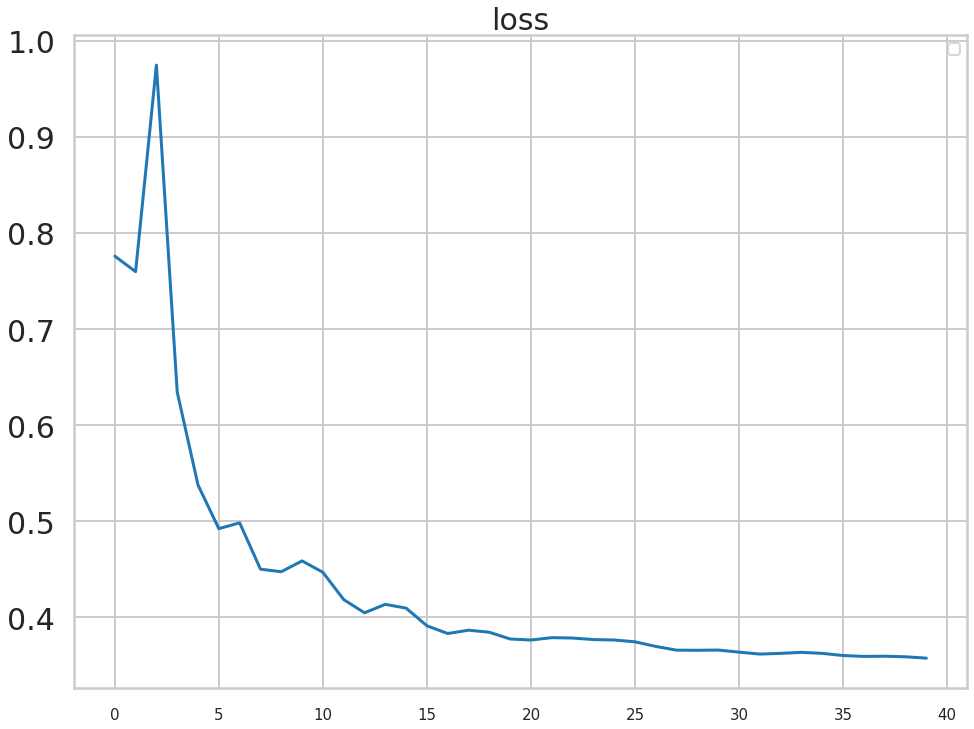
\includegraphics[width=0.4\columnwidth]{./img/lstm_with_arima_loss.png}
	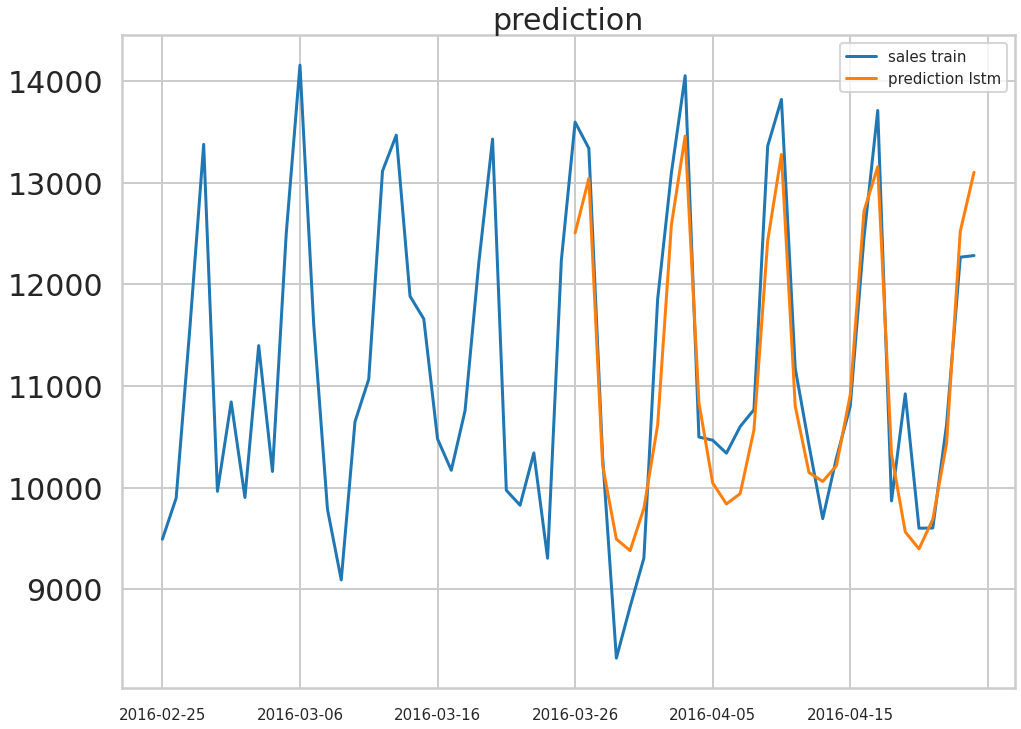
\includegraphics[width=0.4\columnwidth]{./img/lstm_with_arima_prediction.png}
	\caption{Кривая потерь и предсказание LSTM-сети c использованием результатов предсказаний ARIMAX модели}
	\label{img:lstm_with_arima_forecast}
\end{figure}

Результаты предсказаний с помощью модели LSTM очень похожи на результаты предсказаний
с помощью SARIMAX. Стоит заметить, что LSTM была обучена и вычислялась с помощью GPU.
В то время как оптимизация параметров модели SARIMAX производились на процессоре и
для получения примерно одинаковых результатов требовалось столько же времени.
Если бы LSTM обучалась на процессоре, время обучения бы исчислялось не секундами, а часами,
так как это затратный по вычислительным мощностям процесс.

В результате эксперимента была обучена LSTM сеть с размерностью скрытого слоя равной 200.
Результат обработки LSTM-сети после ее вычислений попадал в полносвязную сеть с размерностью
тоже 200. Кривая потерь в процессе обучения и график с предсказаниями представлены не графиках \ref{img:lstm_forecast}.
Значение $ RMSSE = 0.000167 $. Это немного меньше, чем у модели SARIMAX, но незначительно.

Кроме того, важным недостатком такой модели может быть то, что она не
способна предсказывать данные из новой области значений.
Для того, чтобы предсказать временной ряд с трендом, нужно или делать
декомпозицию или преобразовать исходный ряд так, чтобы в нем не было тренда.
После того, как получили предсказания, нужно проделать обратные преобразования.
Это не всегда удобно. Возможно, этого недостатка можно избежать,
если использовать модифицированную LSTM. Предположительно, если не использовать
функции активации, то такой проблемы не будет. Но у такой модели
в некоторых случаях больше вероятность получить взрыв градиентов, когда
веса сети будут слишком большими. Такая ситуация ведет к невозможности обучить модель.


\def\figurename{Рис}
\begin{figure}[t]
	\centering
	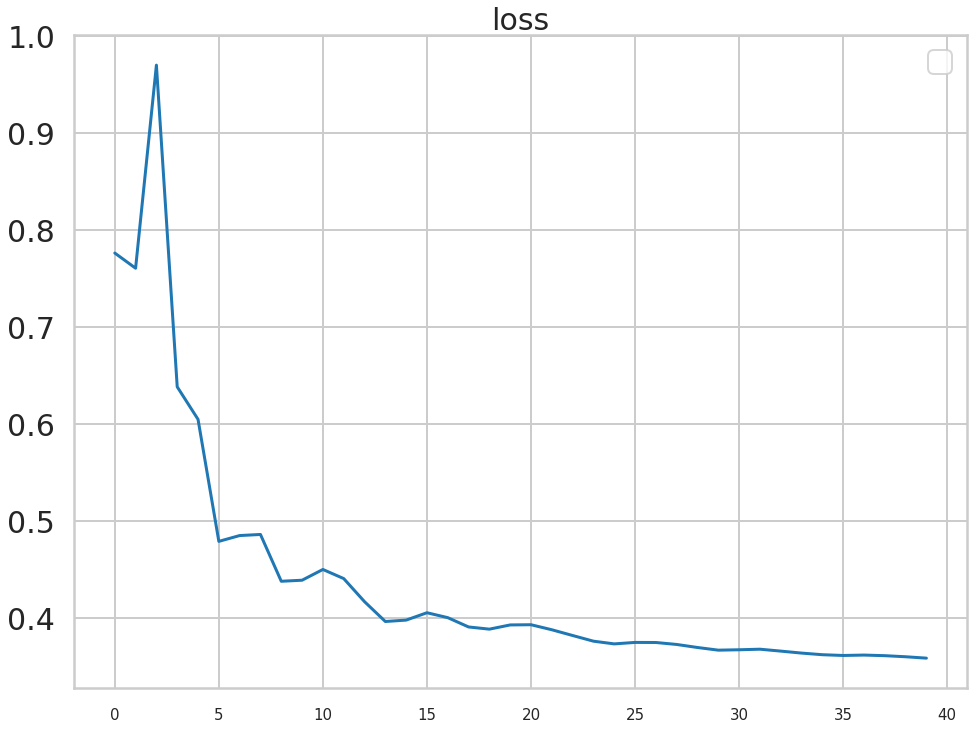
\includegraphics[width=0.4\columnwidth]{./img/lstm_loss.png}
	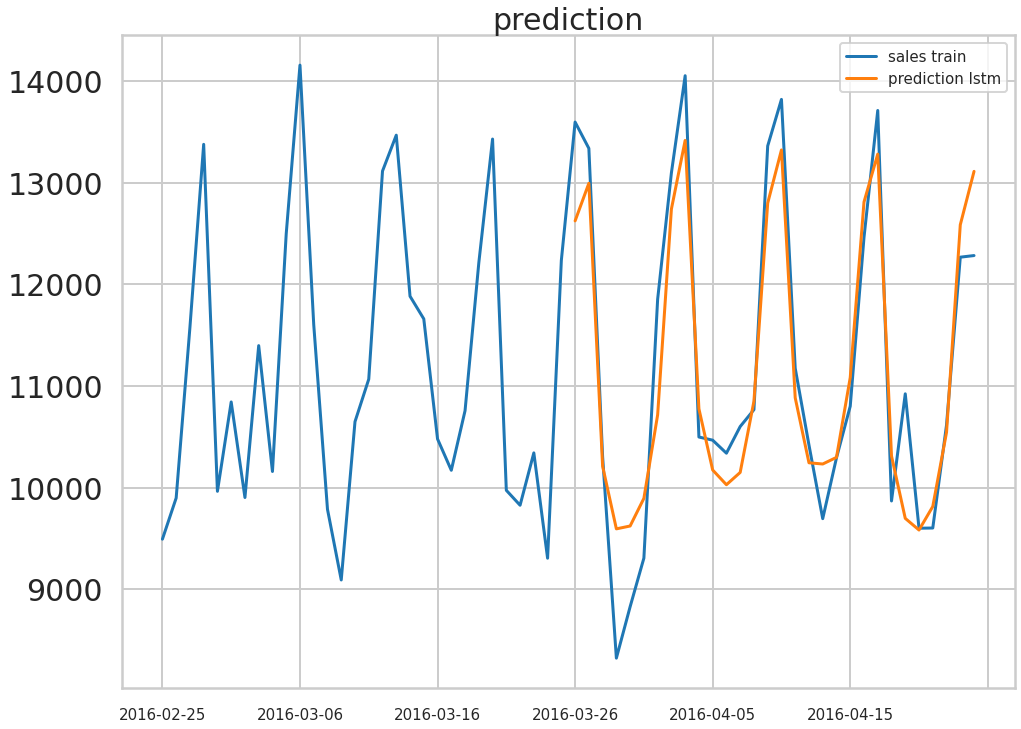
\includegraphics[width=0.4\columnwidth]{./img/lstm_prediction.png}
	\caption{Кривая потерь и предсказание LSTM-сети}
	\label{img:lstm_forecast}
\end{figure}

\section{Построение модели FCM-LSTM}

Данная модель разрабатывалась с использованием фреймворка $ pytorch $.
Для исследования модели была построена карта \ref{img:fcm_lstm_map}.
Данные были разбиты на 9 временных рядов. Они были сгруппированы по
магазину и по категории. Экзогенные переменные не использовались,
так как для данной задачи не было найдено таких экзогенных параметров,
которые могли бы значительно повлиять на краткосрочные предсказания.

В качестве модели в вершине карты были использованы сети LSTM с размерностями
внутреннего состояния равными 50, 100, 200, 300. Каждая модель обучалась 40 эпох.
С увеличением размерности скрытого состояния увеличивалось и время обучения.

Наилучшее значение $ WRMSSE $ было получено для модели с размерностью 50 \ref{tbl:rmsse_fcm_lstm}.
Веса ошибок каждого ряда были взяты единичные, так как ошибки для всех рядов расцениваются одинаково.
Можно заметить, что слишком большие значения размерности скрытого состояния модели
привели к ухудшению метрики $ WRMSSE $. Это можно объяснить слишком сложной моделью.
Не смотря на это, прогнозы исследуемых моделей отличаются незначительно.
Поэтому разница в значениях ошибки предсказаний может быть даже просто случайной.
Но по сравнению с моделью чистой LSTM и чистой ARIMAX, данная модель показала худшие результаты.
Но зато модель с когнитивной картой может предсказывать разные временные ряды отдельно.
Для сравнения предсказаний данной модели с моделями $ LSTM $ или $ SARIMAX $, в
таблице представлен столбец со значением $ RMSSE $ для суммы предсказанных рядов
по всем категориям и всем магазинам. Ошибка оказалась больше, чем у  $ LSTM $ и $ SARIMAX $
моделей.

\begin{table}
    \caption{Зависимость $ WRMSSE $ и $ RMSSE $ для суммы рядов в зависимости от размерности скрытого состояния сети }
    \centering
    \begin{tabular}{|l|r||r|r|}
        \hline
            Размерность скрытого слоя &   WRMSSE & RMSSE of sum \\
        \hline
            50                         & 0.000370 & 0.000242 \\
            100                        & 0.000405 & 0.000243 \\
            200                        & 0.000388 & 0.000226 \\
            300                        & 0.000416 & 0.000237 \\
        \hline
    \end{tabular}
    \label{tbl:rmsse_fcm_lstm}
\end{table}

Результаты предсказаний модели с $ hidden\_size = 200 $ представлены на графике \ref{img:prediction_fcm_lstm}.
Можно заметить, что ряды с малыми колебаниями данная модель предсказывает плохо.
Результаты предсказания выглядят сглаженными. Это можно объяснить тем, что
в данных есть выбросы (например, нет продаж на каждое Рождество).
Для того, чтобы избежать этой проблемы, можно просто исключить  выбросы из выборки.
Или обучить модель на том участке данных, на котором выбросов нет.
Уменьшение размера выборки может улучшить результат предсказаний для любой модели.
Так как если данных очень много, то слишком старые показатели временного ряда
могут быть не так полезны для модели, потому что более актуальная информация
о процессе будет содержаться в части ряда, которая ближе к промежутку, который
требуется предсказать.
Кроме того, для борьбы с выбросами можно бороться и другими методами.
Можно прологарифмировать ряд. Но такое преобразование сгладит пики при больших значениях
временного ряда. И при обратном преобразовании маленькие отклонения исходного ряда
могут превратиться в гигантские скачки или выбросы.
Использование экзогенных параметров, таких как индикатор Рождества, не позволило бы
справиться с проблемой.

Результаты предсказаний для карты с размерностью скрытого состояния 200, обученной на 110 предшествующих днях
представлены на графиках \ref{img:prediction_fcm_lstm_110d}.

\def\figurename{Рис}
\begin{figure}[t]
	\centering
	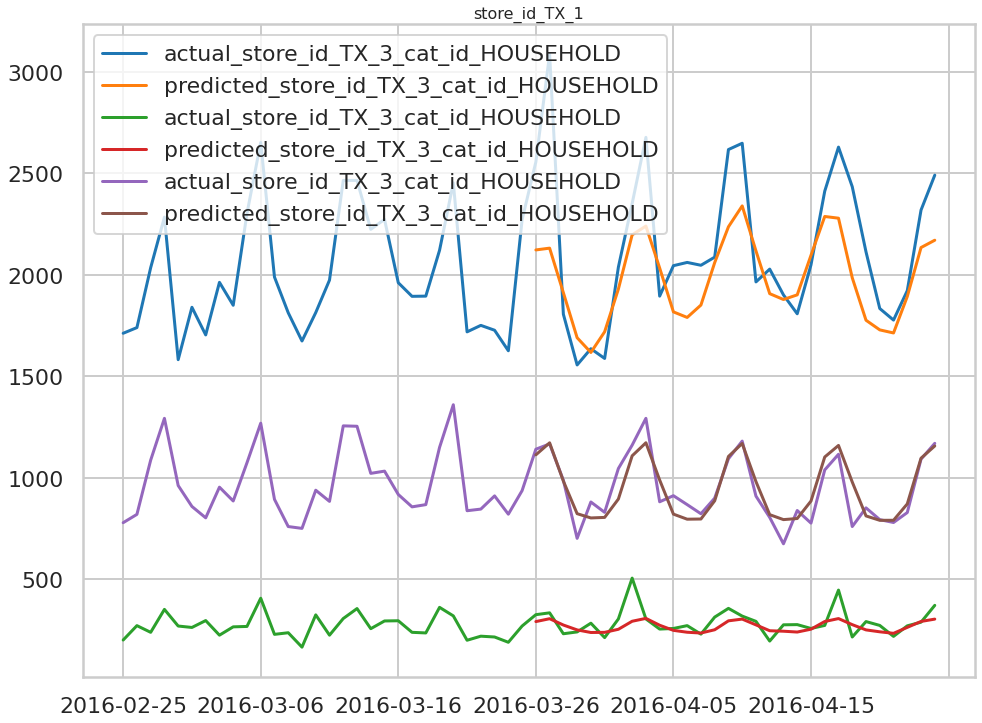
\includegraphics[width=0.25\columnwidth]{./img/fcm_lstm_tx1.png}
	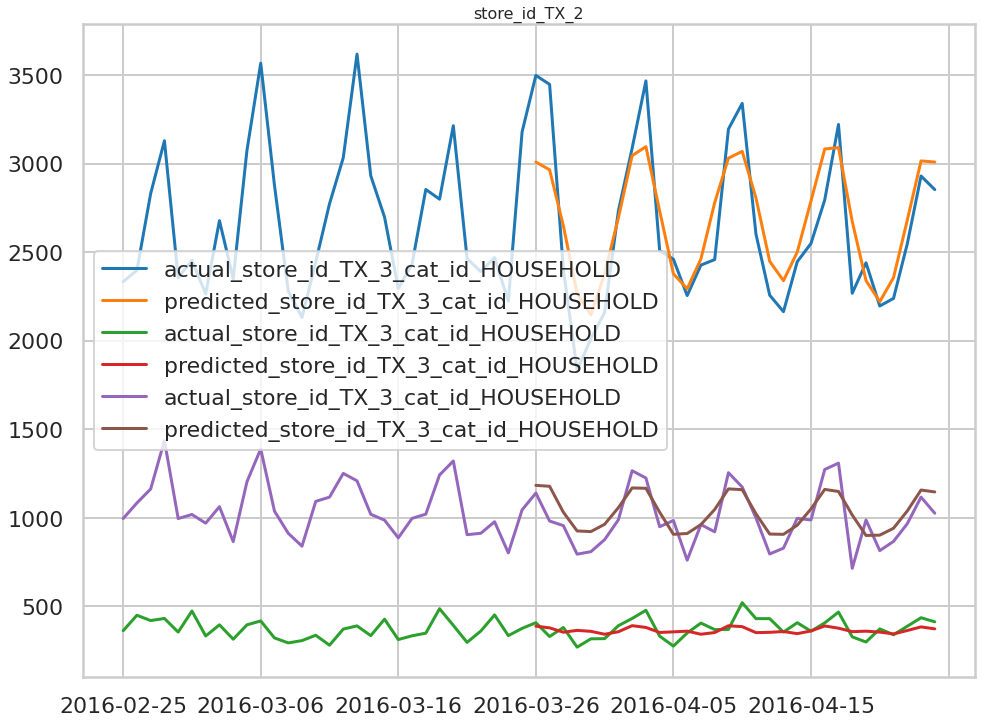
\includegraphics[width=0.25\columnwidth]{./img/fcm_lstm_tx2.png}
	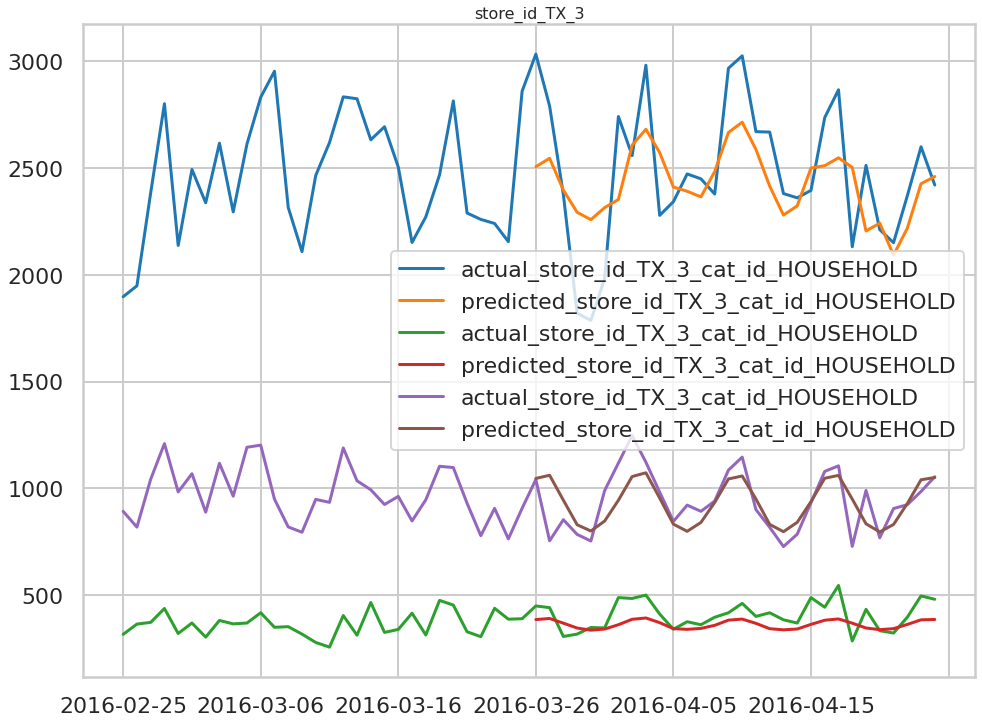
\includegraphics[width=0.25\columnwidth]{./img/fcm_lstm_tx3.png}
	\caption{Предсказания по каждой категории товара для каждого магазина с помощью FCM-LSTM с размерностью скрытого состояния 200, обученной на выборке с выбросами}
	\label{img:prediction_fcm_lstm}
\end{figure}


\def\figurename{Рис}
\begin{figure}[t]
	\centering
	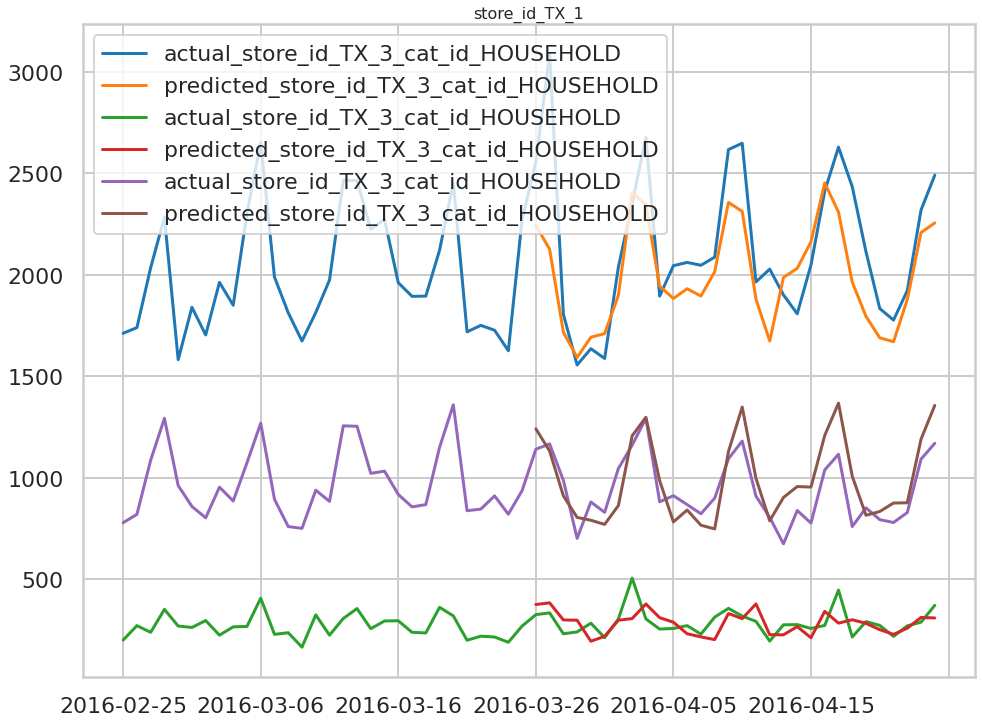
\includegraphics[width=0.25\columnwidth]{./img/fcm_lstm_tx1_110_days.png}
	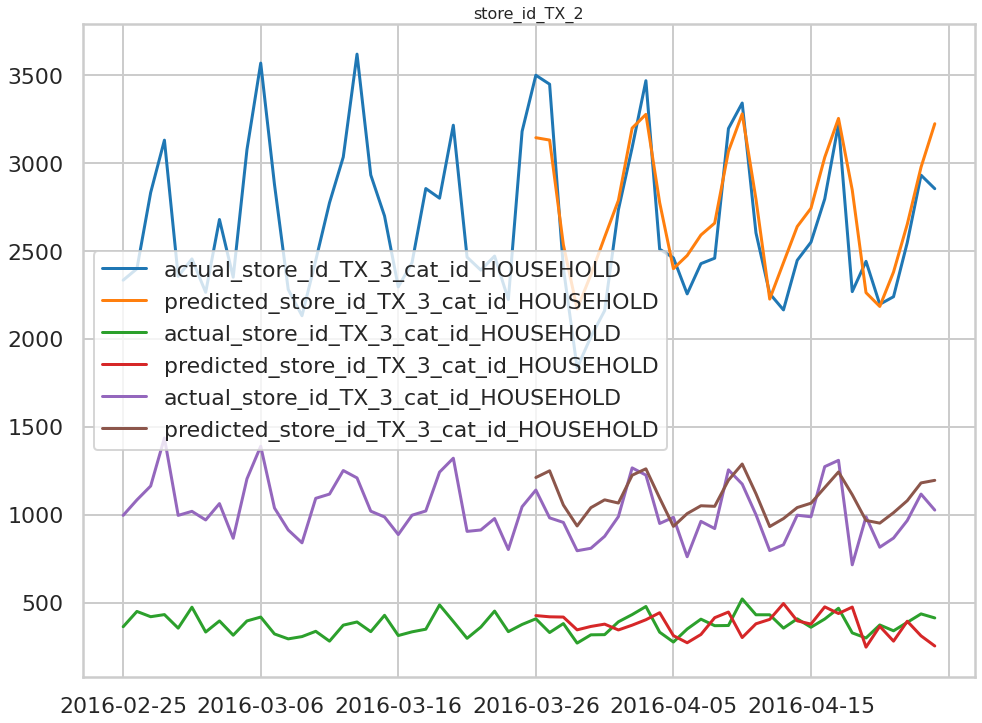
\includegraphics[width=0.25\columnwidth]{./img/fcm_lstm_tx2_110_days.png}
	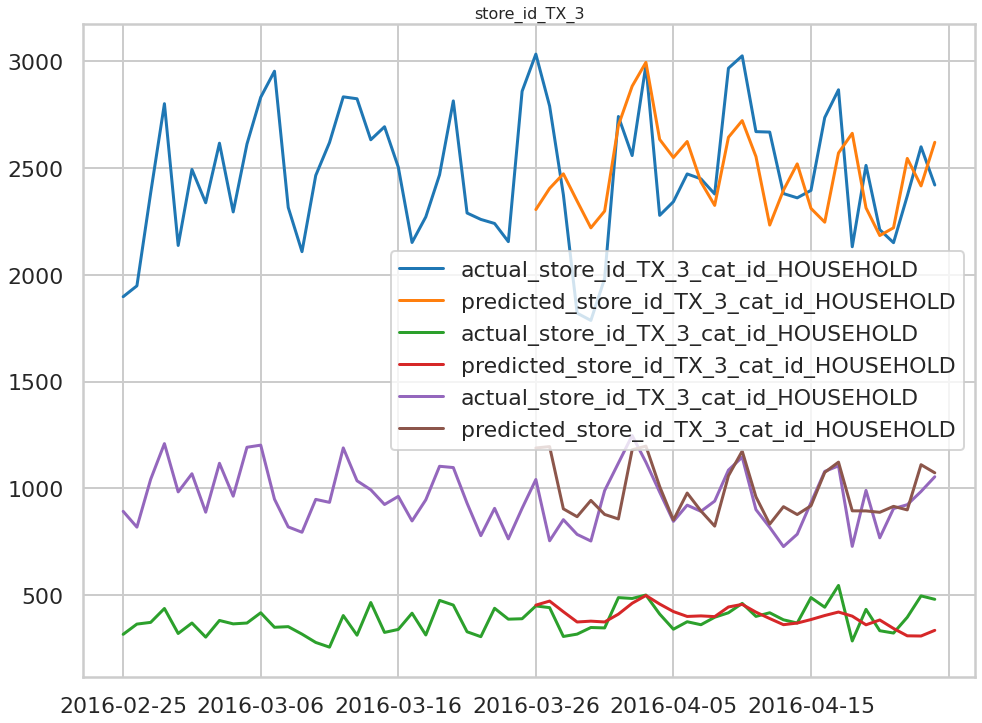
\includegraphics[width=0.25\columnwidth]{./img/fcm_lstm_tx3_110_days.png}
	\caption{Предсказания по каждой категории товара для каждого магазина с помощью FCM-LSTM с размерностью скрытого состояния 200, обученной на выборке без выбросов}
	\label{img:prediction_fcm_lstm_110d}
\end{figure}


В таблице \ref{tbl:all_models_comparation} приведены ошибки для всех исследуемых типов моделей.
Эксперимент был проведен еще раз для каждой модели. Следует отметить, что при повторном
запуске значения ошибок могут варьироваться. Это объясняется тем, что некоторые веса
в нейросетевых методах инициализируются случайным образом. Значения ошибок представленных
в этой таблице можно считать средними.

\begin{table}
    \caption{ Ошибки в предсказании общего количества продаж на 30 дней для исследованных типов моделей }
    \centering
    \begin{tabular}{|l|r||r|}
        \hline
            Модель                                                            & RMSSE     & MSE    \\
        \hline
            SARIMAX(2, 0, 3)x(0, 1, 1, 7) с эндогенными переменными           & 0.0002077 & 526786 \\
            LSTM (hidden\_size = 200)                                         & 0.0002312 & 398844 \\
            FCM-LSTM (hidden\_size = 200), обученная на выборке с выбросами   & 0.0002354 & 676686 \\
            FCM-LSTM (hidden\_size = 200), обученная на выборке без выбросов  & 0.0002129 & 553416 \\
        \hline
    \end{tabular}
    \label{tbl:all_models_comparation}
\end{table}

\section{Выводы}

В данной главе была реализована система для нейро-нечетного когнитивного картирования с использованием
методов нейронных сетей, которая удовлетворяет требованиям, определенным в предыдущей главе.

Исследованы самостоятельные модели для прогнозирования временных рядов:
$SARIMAX$, $LSTM$, $SARIMAX + LSTM$.
Исследовано влияние выбросов на предсказание модели и границы применимости каждой модели.
Разработанная модель была сравнена с другими моделями для предсказания временных рядов.
Также описаны инструменты, с помощью которых была реализована система.
Описана структура программного обеспечения, проведено тестирование разработанной системы.

Модель когнитивной карты, обученная на выборке с выбросами, имела самые большие показатели
ошибок. Но такая же модель обученная на выборке без выбросов
оказалась конкурентноспособной с другими моделями, не использующими
когнитивные карты. Но у модели с когнитивной картой есть ряд преимуществ,
описанных во второй и третьей главе данной работы:

\begin{itemize}
	\item Разработанная модель на основе карты более интерпретируема;
	\item Предсказание такой модели более детальное: предсказаны значения каждой категории товаров для каждого магазина;
	\item Больше возможностей для моделирования благодаря простому добавлению новых параметров;
	\item Разработанная модель гибка в плане дообучения;
	\item Для добавления новых параметров системы не требуется полное переобучение модели;
\end{itemize}

Однако есть и недостатки:
\begin{itemize}
	\item Суммарная ошибка по предсказанию общего количества продаж больше,
	чем у методов, которые предсказывают сразу целевое значение объема продаж,
	а не продажи по категориям. Это можно объяснить тем, что количество прогнозируемых рядов больше.
	И ошибки при прогнозировании каждого ряда в сумме получаются больше, чем в предсказаниях
	самостоятельных моделей.
	\item Модель имеет большое количества параметров и требует больших вычислительных мощностей.
	Это ожидаемо, так как такая модель прогнозирует большее количество временных рядов.
	Для предсказания нескольких временных рядов можно использовать и одну LSTM
	сеть. И если сравнивать FCM-LSTM с LSTM для прогнозирования нескольких временных рядов,
	то FCM-LSTM будет требовать меньше ресурсов и будет проще обучаться. Потому что
	в FCM-LSTM строго определены, какие концепты могут влиять друг на друга, а какие --- нет.
	В обычной LSTM для предсказания нескольких временных рядов, будет создано столько весов,
	сколько бы потребовалось для FCM-LSTM в случае, если бы такая карта представляла из себя
	полносвязный граф.
\end{itemize}


